

\documentclass[journal=jacsat,manuscript=article]{achemso}
\usepackage{graphicx}
\usepackage{hyperref}
\usepackage{chemformula} % Formula subscripts using \ch{}
\usepackage[T1]{fontenc} % Use modern font encodings
\newcommand*\mycommand[1]{\texttt{\emph{#1}}}

\author{Damien E. Coupry}
\email{damien.x.coupry@gsk.com}
\affiliation[GlaxoSmithKline]
{GlaxoSmithKline, Data and Computational Sciences, UK}
\author{Peter Pog\'{a}ny}
\affiliation[GlaxoSmithKline]
{GlaxoSmithKline, Data and Computational Sciences, UK}

\title{Application of deep metric learning to molecular  similarity}
\date{\today}

\abbreviations{QSAR, GNN, MPNN, RG, GFRG, DFRG, ECFP}
\keywords{metric learning, similarity, graph neural networks, deep learning}


\begin{document}
\maketitle

\begin{abstract}
Graph based methods are increasingly important in chemistry and drug discovery, with applications ranging from QSAR to molecular generation. Combining graph neural networks and deep metric learning concepts, we expose a framework for quantifying molecular similarity based on learned embeddings separate from any endpoint. Using a minimal definition of similarity, and data from the ZINC database of public compounds, this work demonstrate the  properties of the embedding and its suitability for a range of applications, among them a novel reconstruction loss method for training deep molecular auto-encoders. We also compare the performance of the embedding to standard practices, with a focus on known failure points and edge cases.
\end{abstract}

\section{Introduction}
\paragraph{}
Quantifying the similarity of chemical structures has been a much used tool in drug discovery for decades\cite{willett1998chemical}, and has often been adopted as a design principle for lead optimization \cite{kubinyi1998similarity, maggiora2014molecular}, under the assumption that similar molecules have a higher probability of exhibiting similar properties than dissimilar ones \cite{johnson1990concepts, patterson1996neighborhood, martin2002structurally}. Indeed, the successful use of bioisosterism in drug development makes heavy use of the concept  \cite{patani1996bioisosterism, lima2005bioisosterism}, to the point that similarity is sometimes defined as a consequence of the properties, rather than the cause\cite{bender2004molecular}. Most of the benchmarks for chemical structure similarity rely on this definition to compare methods \cite{irwin2008community, rohrer2009maximum, riniker2013open}, driven in part by the availability of public activity datasets \cite{gaulton2012chembl}. Yet, pitfalls such as so-called ``activity cliffs''\cite{maggiora2006outliers, stumpfe2012exploring, stumpfe2014recent} should moderate the confidence in the underlying principle. Furthermore, other use cases of similarity exist, and are not captured by the similar properties paradigm: patent mining and infringement prediction \cite{rhodes2007mining}, building block selection for synthesis, retrosynthesis and scaffold hopping\cite{bohm2004scaffold, boehm2008similarity, coley2017computer}, molecular generation evaluation\cite{mendez2020novo}, etc. A ``good'' measure of similarity should ideally show equal performance in all these applications, never relying too much on any one definition or type of benchmark.
\paragraph{}
On the practical side, similarity can be more generally understood as the combination of a molecular representation and an appropriate metric\cite{maggiora2014molecular}. Today, the combination of two-dimensional molecular circular fingerprints \cite{cereto2015molecular, rogers2010extended} with the Tanimoto coefficient \cite{bajusz2015tanimoto} is still the most widely used, and  generally hard to outperform in traditional benchmarks\cite{raymond2002effectiveness}. Still, these methods suffer from a number of identified drawbacks, regularly analysed but difficult to route around in the absence of a more general representation\cite{flower1998properties, dixon1999hidden}. Most of the recent efforts to develop original molecular encodings focus on the relational nature of molecules as seen in a 2D context. By considering structures as a graph with atoms as nodes and bonds as edges, we can draw on the considerable field of extant work on graph similarity in general: computationally expensive graph edit distance, graph isomorphism quantification or maximum common subgraph \cite{garcia2019ligand, bunke1998graph, bunke1983inexact, dijkman2009graph, berretti2001efficient}, graph kernels for similarity \cite{kriege2020survey}, and the increasingly popular deep learning algorithms\cite{ma2021deep}. The latter rely on embeddings learned from variational reconstruction tasks\cite{jin2018junction}, end-to-end property predictions \cite{brown2009chemoinformatics}, or borrow architectures from facial recognition \cite{bai2019simgnn}.
\paragraph{}
In this work, we leverage  the ability of graph neural networks from the Deep Graph Library\cite{wang2019deep, li2021dgl} to learn chemical structures embeddings using the triplet loss\cite{schultz2004learning}, to our knowledge the first such use of it. A training dataset is constructed automatically using a minimal definition of molecular similarity and public compounds. We show that these embeddings satisfy the conditions to be considered an improved encoding of chemical information in both traditional benchmarks and novel applications.


\section{Experiments}\label{experiments}
\subsection{Dataset generation}

The ZINC database was downloaded (1.487 billion compounds)\cite{ZINC15,ZINC_db} and processed as follows. Parent structures were created, bad valencies, compounds with poorly defined bonds, isotope labelled compounds and compounds containing elements other than N, O, C, S, F, Cl, Br and I were removed. This initial filtering removed around 2 million compounds. Reduced Graphs\cite{RedGraph2003,RedGraph2004}, Bemis-Murcko graph and detailed frames\cite{BemisMurcko} were generated for each compound. In the Reduced Graph, the full molecular graph is reduced to pharmacophore feature type nodes. Whereas the Bemis-Murcko graph frames contain the anonymous frame of the molecule without the side chains, atom types and bond orders. The Bemis-Murcko detailed frame contains the frame of the molecule (side chains removed) with atom types and bonds marked. Comparison of these molecular representations is given on Figure~\ref{fig:GF_DF_RG}. 

\begin{figure}[hbtp]
\centering
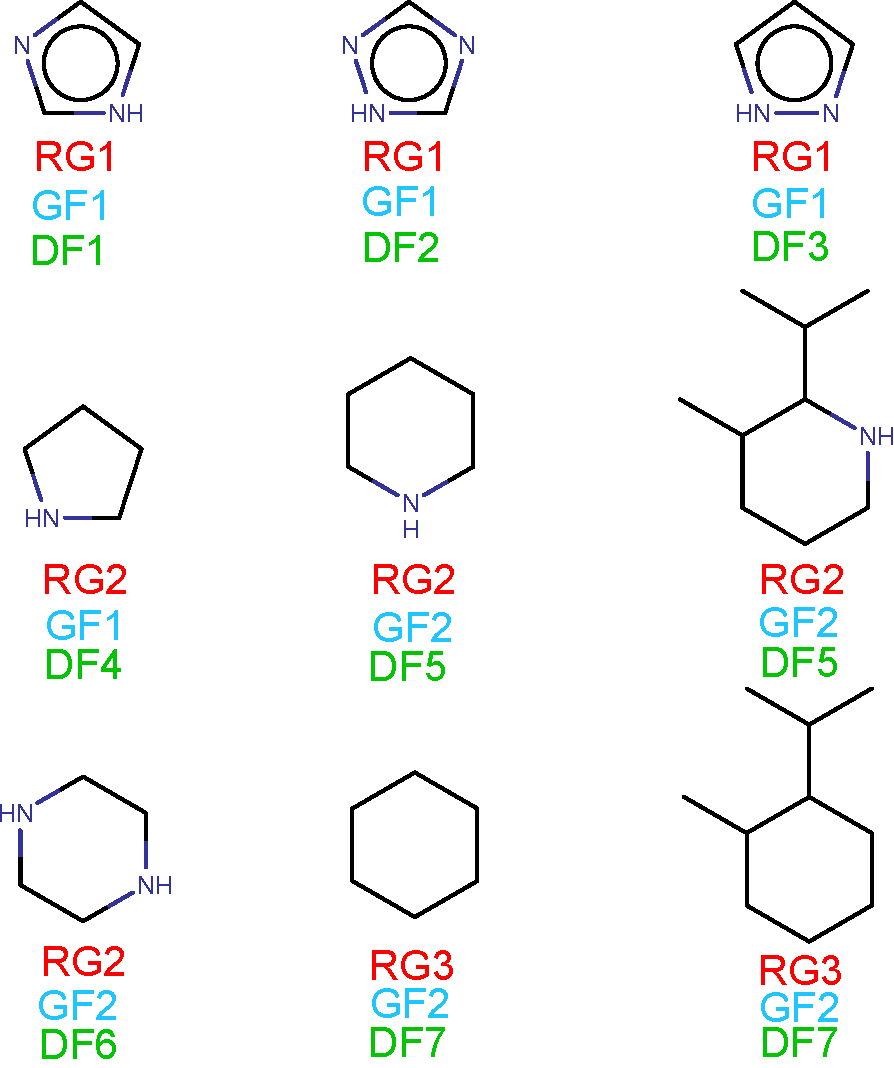
\includegraphics[width=0.5\textwidth]{data/GFRGDF.pdf}
\caption{A comparison of the Reduced Graph (RG), Bemis-Murcko graph (GF) and detailed frames (DF) clusters. The numbers after the character show the cluster. RG1 is a cluster of aromatic ring containing compound which contain hydrogen bond donor and acceptor. RG2 are aliphatic rings with hydrogen bond donors, RG3 are aliphatic rings without feature. There are only two graph frame clusters: 5-membered rings (GF1) and 6-membered rings (GF2). Detailed frames are only identical, if the compounds differ in ring substituents connected to rings with single bonds (DF5 and DF7).}
\label{fig:GF_DF_RG}
\end{figure}

REOS\cite{Walters1998} and PAINS~A\cite{Baell2010} filters were applied on the remaining compounds and molecular weight (MW) was calculated to remove everything with MW$>$650 daltons, thus keeping 1.199 B compounds. Compounds were clustered in three ways:
\begin{enumerate}
\item Having the same Reduced Graph and Graph Frame (GFRG)
\item Having the same Reduced Graph and Detailed Frame (DFRG)
\item  Having the same Reduced Graph (RG)
\end{enumerate}
Most of the processing after this was done using BIOVIA Pipeline Pilot\cite{biovia2020}. All compounds belonging to a GFRG cluster with less than 4 members were removed. In the case of compounds belonging to GFRG clusters with more than 10k members, DFRG clusters were used in place of GFRG. For DFRG clusters, a maximum size of 20k members was established, with random subsampling performed on clusters above this limit. 1.13 billion compounds remained and cluster centers were assigned to them. Cluster Molecules component of BIOVIA Pipeline Pilot\cite{biovia2020} was used to determine the cluster centroids for each cluster defined above (ECFP4 and heavy atom count was used for getting the centroids). For every cluster the number of identities was calculated. If the number of identities was larger than 0.4, all the cluster elements were discarded. 1.113 billion compounds remaind in 16.71 million clusters. The number of clusters for each Reduced Graph was calculated and only Reduced Graphs which have at least 2 clusters were kept (1.059 billion compounds).

The triplet loss trains networks by contrasting a reference structure with two additional compounds, called positive and negative controls. The positive control should be qualitatively similar to the reference. For this purpose, the two were selected randomly from within the same cluster (GFRG cluster for the initial smaller clusters, for the larger clusters, where GFRF cluster size~$\geq$~10,000, DFRG clusters are used). The negative control should conversely be less similar to the reference than the positive. Selecting a very different compound is not optimal, since the chemical space size increase towards larger dissimilarities. Thus, while it would be correct to choose a negative control from a different cluster, choosing a compound that has \textit{some} similar features to the reference is more valuable to the training process. Therefore we have randomly selected the negative control from a different cluster than the cluster of the reference, but their Reduced Graph should be the same. This way 12'361'633 triplets were created. A detailed schema of the data preparation can be seen on Figure~\ref{fig:Process_Diagram}.

\begin{figure}[hbtp]
\centering
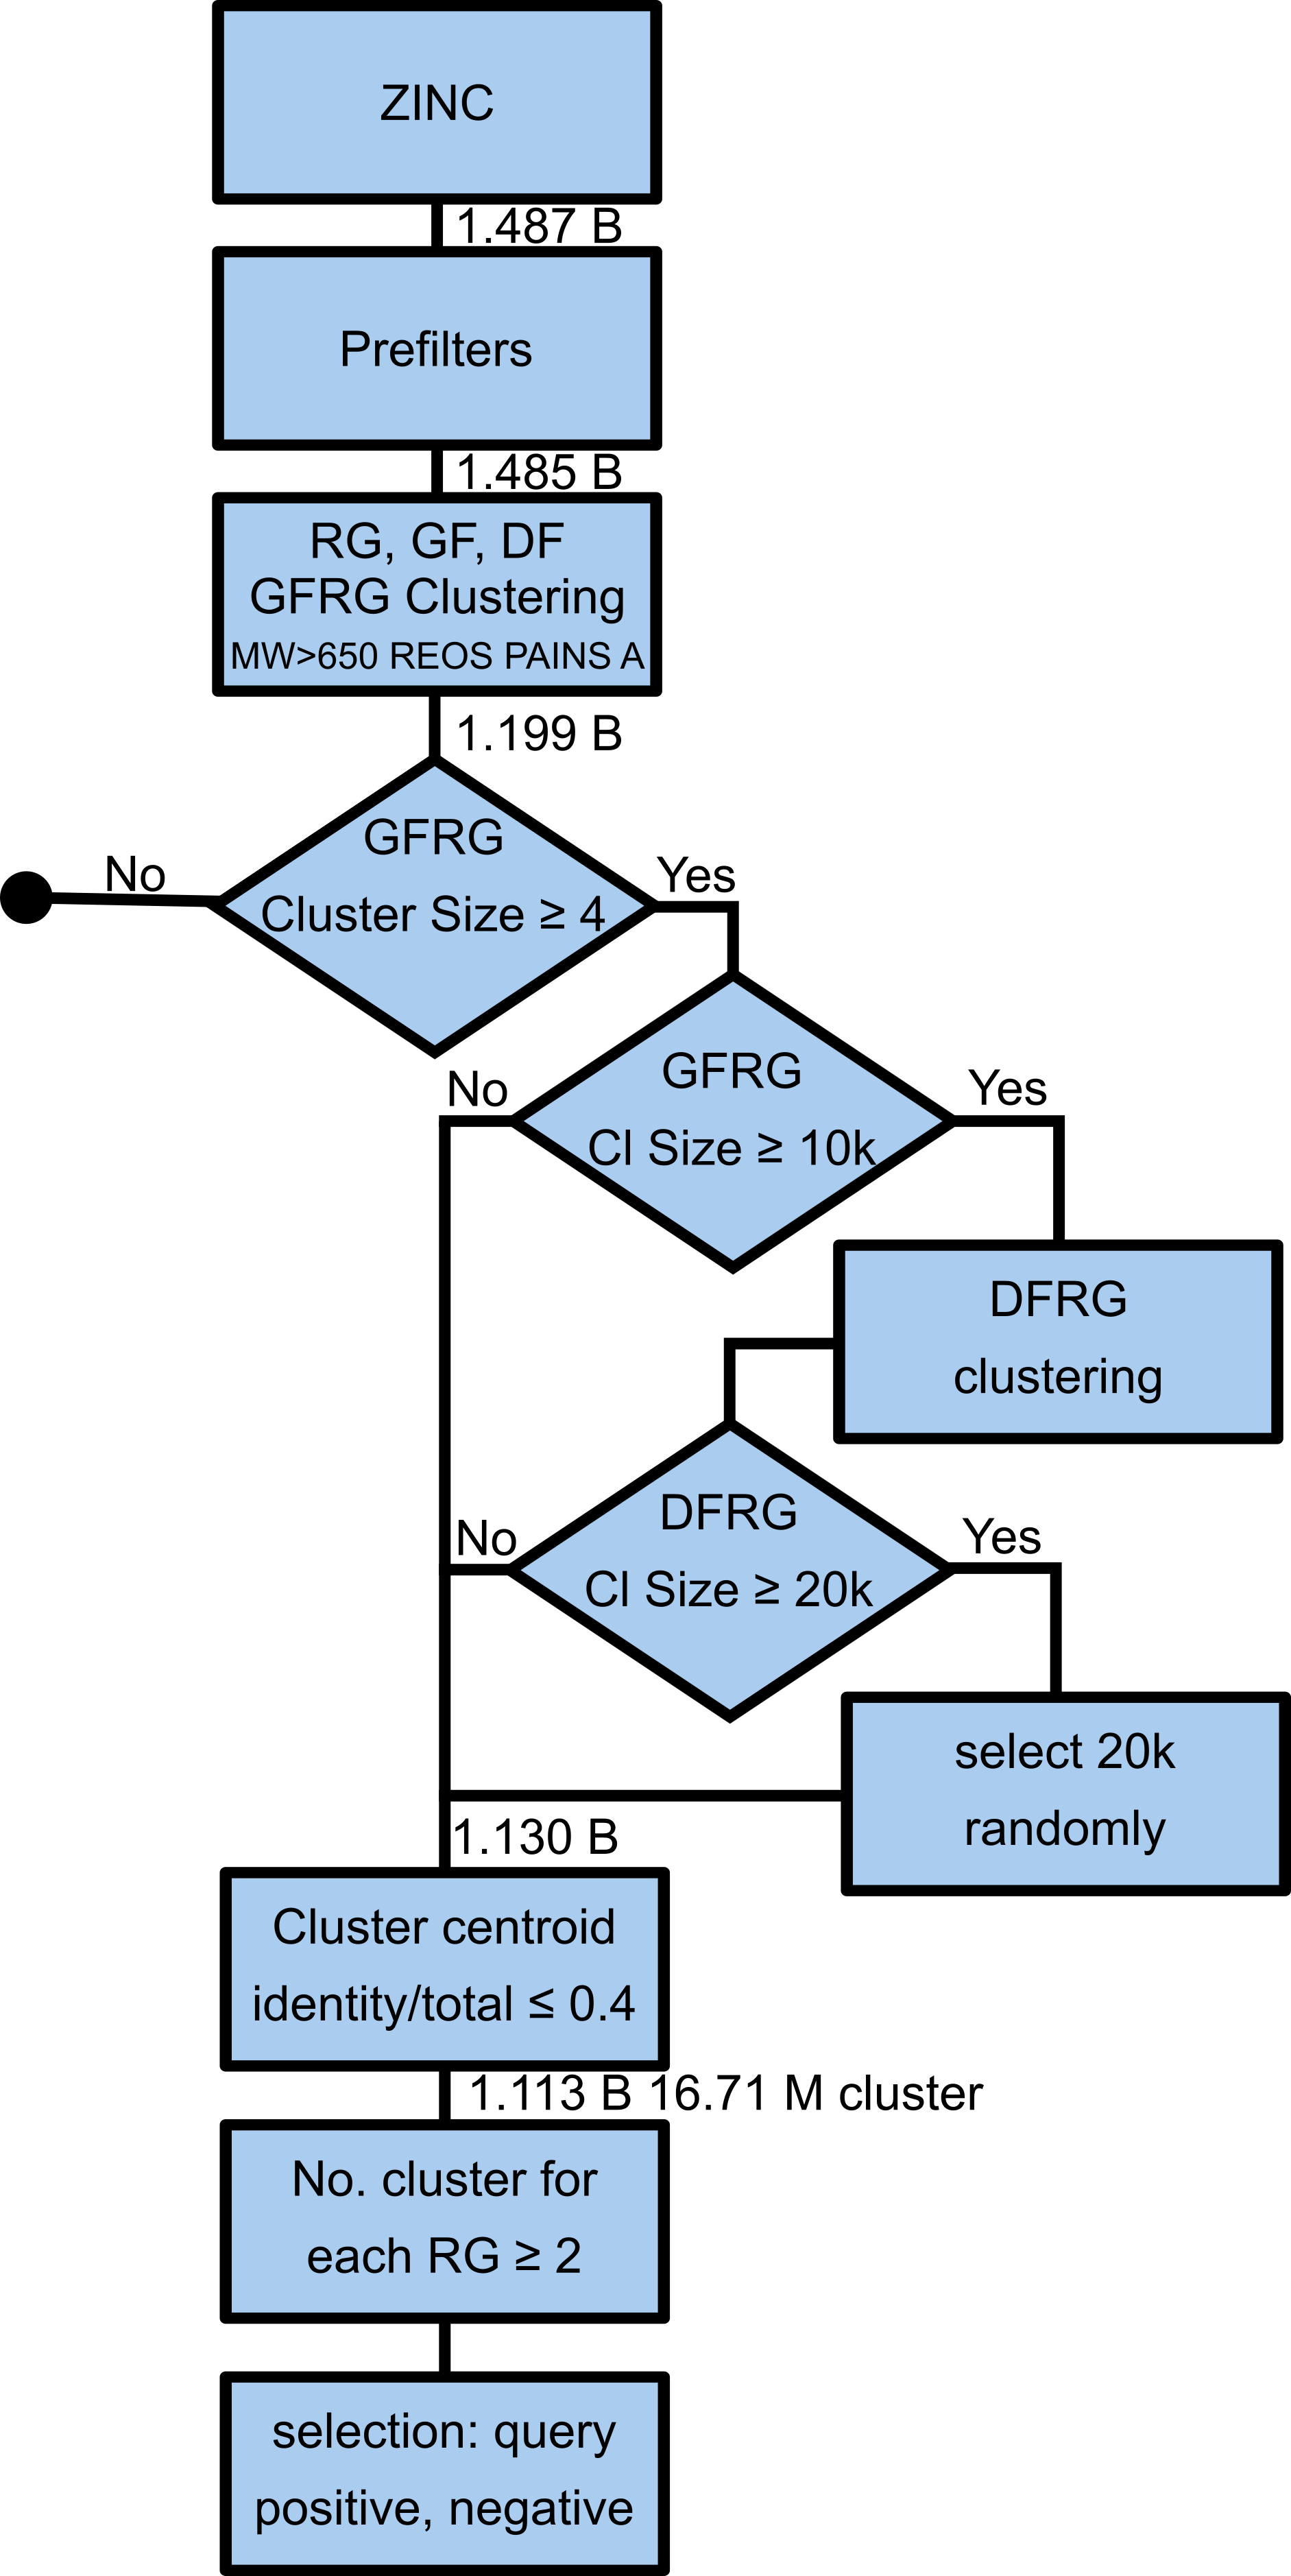
\includegraphics[width=0.5\textwidth]{data/Process_Diagram.png}
\caption{The process diagram of data preparation.}
\label{fig:Process_Diagram}
\end{figure}

\subsection{Model training}
For all training and benchmarking purposes, the random seed is fixed at 42 for repeatability, and the hyperparameters have been kept unoptimized and to the default values to prevent bias. We used the DGL-Lifesci open source framework for computations on graphs, and its message passing neural network implementation (MPNNPredictor)\cite{gilmer2017neural} as model architecture. This type of model repeatedly accumulates bond information as well as node information based on connectivity, and has been used with great effect in state of the art QSAR applications \cite{yang2019analyzing}. We chose to use the default parameters and an output size equal to 16 as an embedding dimension (\textit{n\_tasks}). The input for such a model are molecular graphs, which are obtained using the CanonicalAtomFeaturizer and CanonicalBondFeaturizer from DGL. The details of what is included in the graphs features can be found in the DGL-lifesci documentation\cite{CanonicalAtomFeaturizer, CanonicalBondFeaturizer}. These representations are regularized with a node ablation probability of 1\% and edge ablation probability of 5\%. At each step of the training, an instance of the MPNN is used to embed each of the three graphs of the input (anchor, positive and negative); the triplet margin loss from pytorch\cite{NEURIPS2019_9015} then updates the weights of the network to maximize the distance between the anchor and negative, while minimizing the distance between the anchor and the positive, as seen in Figure~\ref{fig:triplet_arch}.


\begin{figure}[hbtp]
\centering
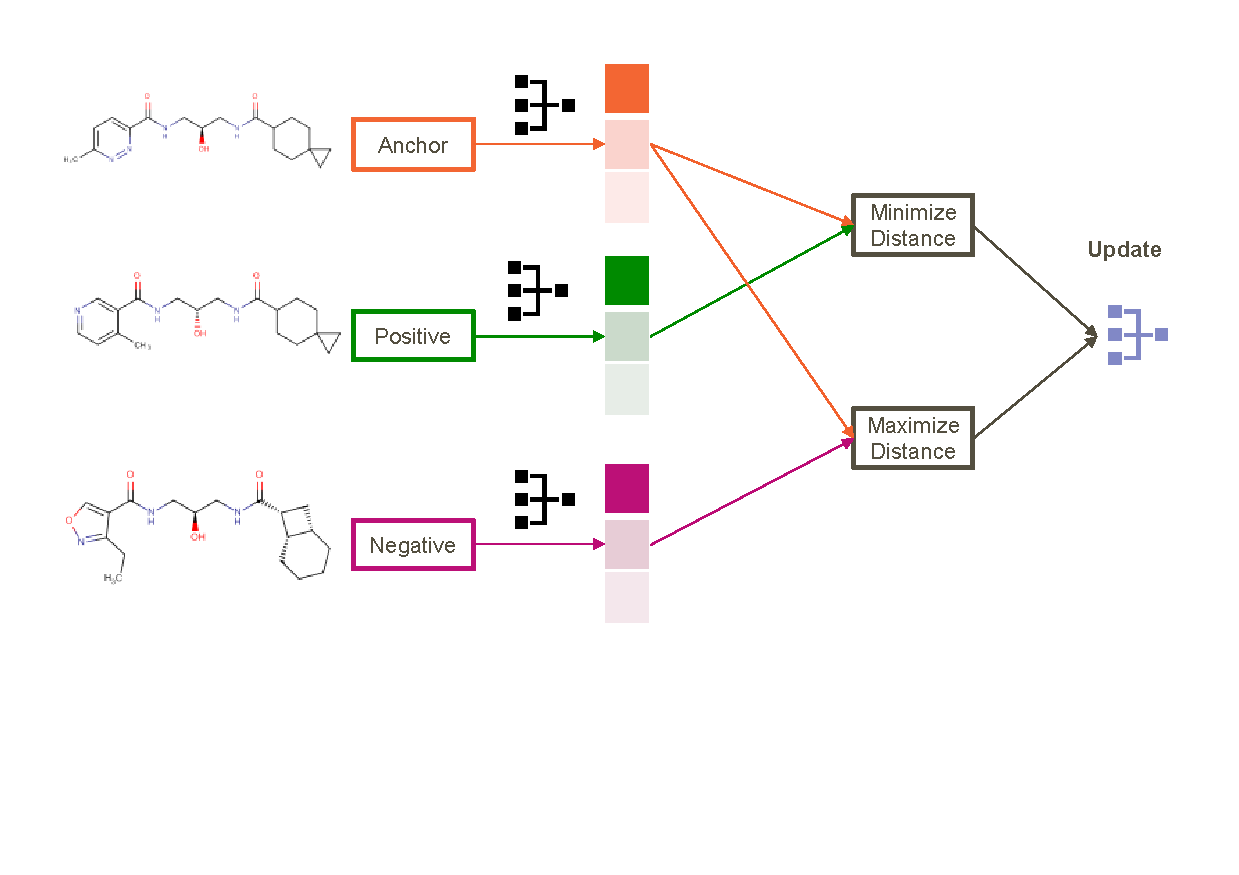
\includegraphics[width=\textwidth, trim={0 4cm 0 0},clip]{data/triplet_network.pdf}
\caption{The architecture of the triplet loss embedding during training.}
\label{fig:triplet_arch}
\end{figure}


 The training used the pytorch-lightning framework \cite{falcon2019pytorch} with a 25 epochs early stopping criterion, the Adam optimizer with the default learning rate of $10.0^{-3}$, and took two days on an Nvidia GEFORCE1080 GPU with a batch size of 128. For more details, hyperparameters, and training curves, please refer to the project's github page.
\subsection{Benchmarks choice}
The benchmarks for the present use case should optimally measure a number of things:
\begin{itemize}
\item The performance on popular applications; here the activity classification tasks such as the ones described in Riniker \textit{et al}\cite{riniker2013open}.
\item The performance on edge cases, such as the ones described in Flower \textit{et al}\cite{flower1998properties}, particularly when the failure of traditional fingerprint based similarity measure is due to the basic technique of fragmentation.
\item The condition of graph isomorphism: the ordering of the molecule atoms and bonds should have no influence on the embedding.
%\item The information density of the embedding, compared to traditional circular fingerprints
\end{itemize}
Additionally, \textit{desired} properties of an encoding come from the coupling with a metric. In particular, using a euclidean distance metric on a well defined euclidean vector space gives rise to a number of interesting properties:
\begin{itemize}
\item very fast querying and operations
\item Similarity can be defined with respect to geometric elements: around a barycentre, along a path between molecules, within a cone, etc.
\item the space and metric together are unbound in value for dissimilarity: there are many more ways of being dissimilar than similar, and the distances distribution could reflect that.
\end{itemize}
\section{Results}\label{results}
\subsection{Activity prediction tasks benchmarking}
While an imperfect measure of fitness for any new chemical embedding, the dominance of benchmarking platforms making use of a variety of activity prediction datasets makes it an obligatory step in evaluating any new contribution. In particular, it enables two separate conclusions to be reached:
\begin{enumerate}
\item Whether the information contained in the embedding is sufficient to fit models successfully, regardless of compared performance
\item Whether these models are statistically different from references to demonstrate the originality of the embedding
\end{enumerate}

To answer the second query, it is necessary to benchmark models on a suitably high number of instances for each class. For this purpose, a dataset of IC50 activities was extracted from the ChEMBL28 database. All targets with a unique structure count between 5k and 20k were kept, with activity threshold automatically set at the 75th percentile of the PIC50 values if and only if this is superior by at least one standard deviation from the minimum value and maximum value. This classification task was modelled by a k-nearest neighbours classifier from the scikit-learn python package\cite{scikit-learn}, trained on ECFP0 and ECFP4 fingerprints from the rdkit package\cite{LandrumRDKit}, as well as on learned embeddings . Only targets with an ECFP0 5-fold stratified cross validation Cohen's Kappa score above 0.25 were kept, to constrain the benchmark tasks to be relatively hard but tractable, resulting in a set of 55 targets. For each triplet of models, the Cochran's Q test was applied to verify statistical difference. The p-values of 30 tested targets were <0.05 and sufficient to reject the null hypothesis that all the models were equivalent. Subsequent confirmation with pairwise McNemar tests with Bonferroni correction show the embedding models to be the source of the statistical difference, thus answering our second point. The performances on this final set of 30 targets are shown in Figure~\ref{fig:Kappa_ChEMBL}, and answers our first point to our satisfaction.

\begin{figure}[hbtp]
\centering
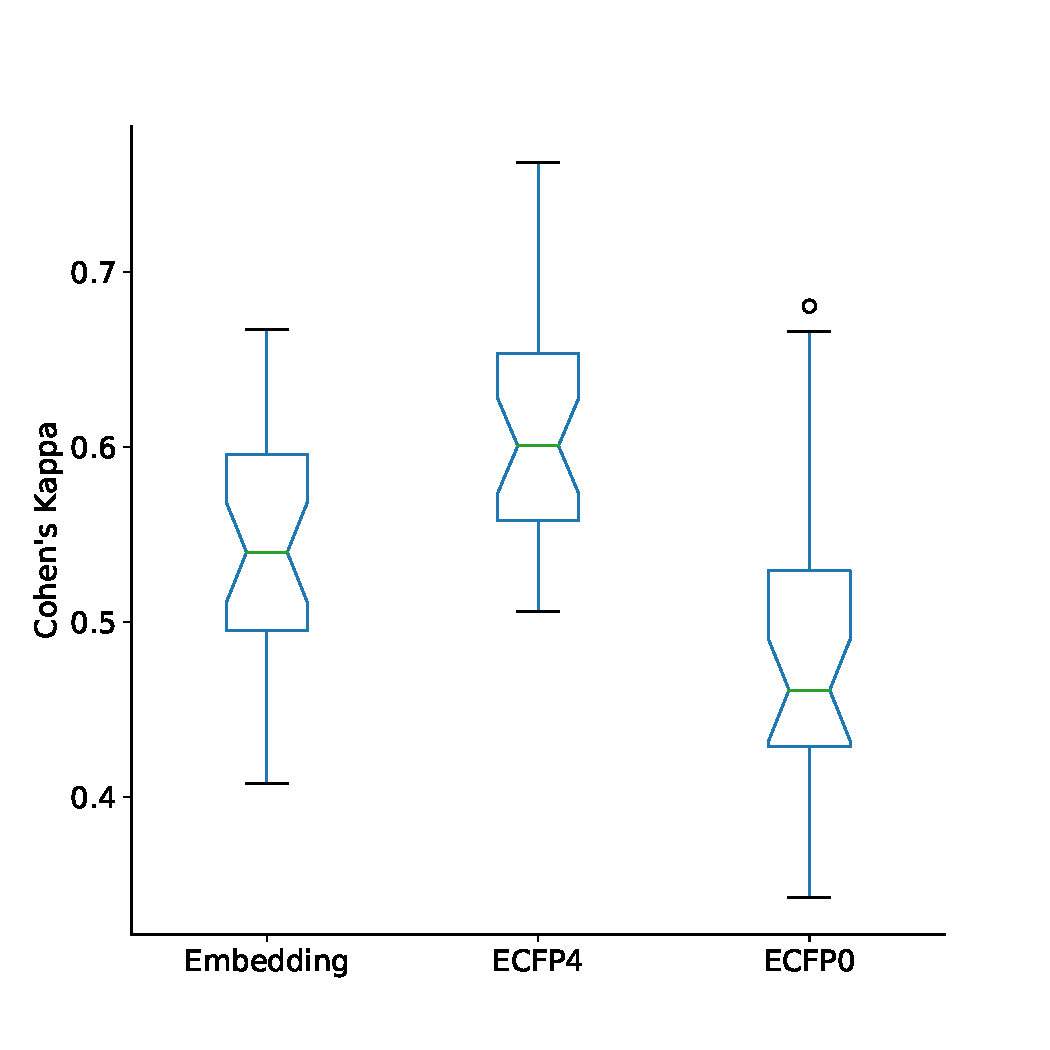
\includegraphics[width=0.5\textwidth]{data/Kappa_ChEMBL.pdf}
\caption{Performance in activity classification tasks from ChEMBL28.}
\label{fig:Kappa_ChEMBL}
\end{figure}


\subsection{Failure points of circular fingerprints}
One noted effect of the bit-string fingerprints is the skewing effect of size on the distribution of similarities as illustrated in Figure~\ref{fig:Similarity_study_cases} of Flowers \textit{et al} \cite{flower1998properties}. Applying the same reference set of compounds for comparison on a diverse set of molecules using the MPNN learned embedding leads to a much better shape of the distributions. While the larger molecule has a more chaotic profile of similarity (probably due to the fact that the larger a structure, the more ways for something to be similar to it), it otherwise seems  independent from the size of the molecules. This is shown in Figure~\ref{fig:References_distributions}.


\begin{figure}[hbtp]
\centering
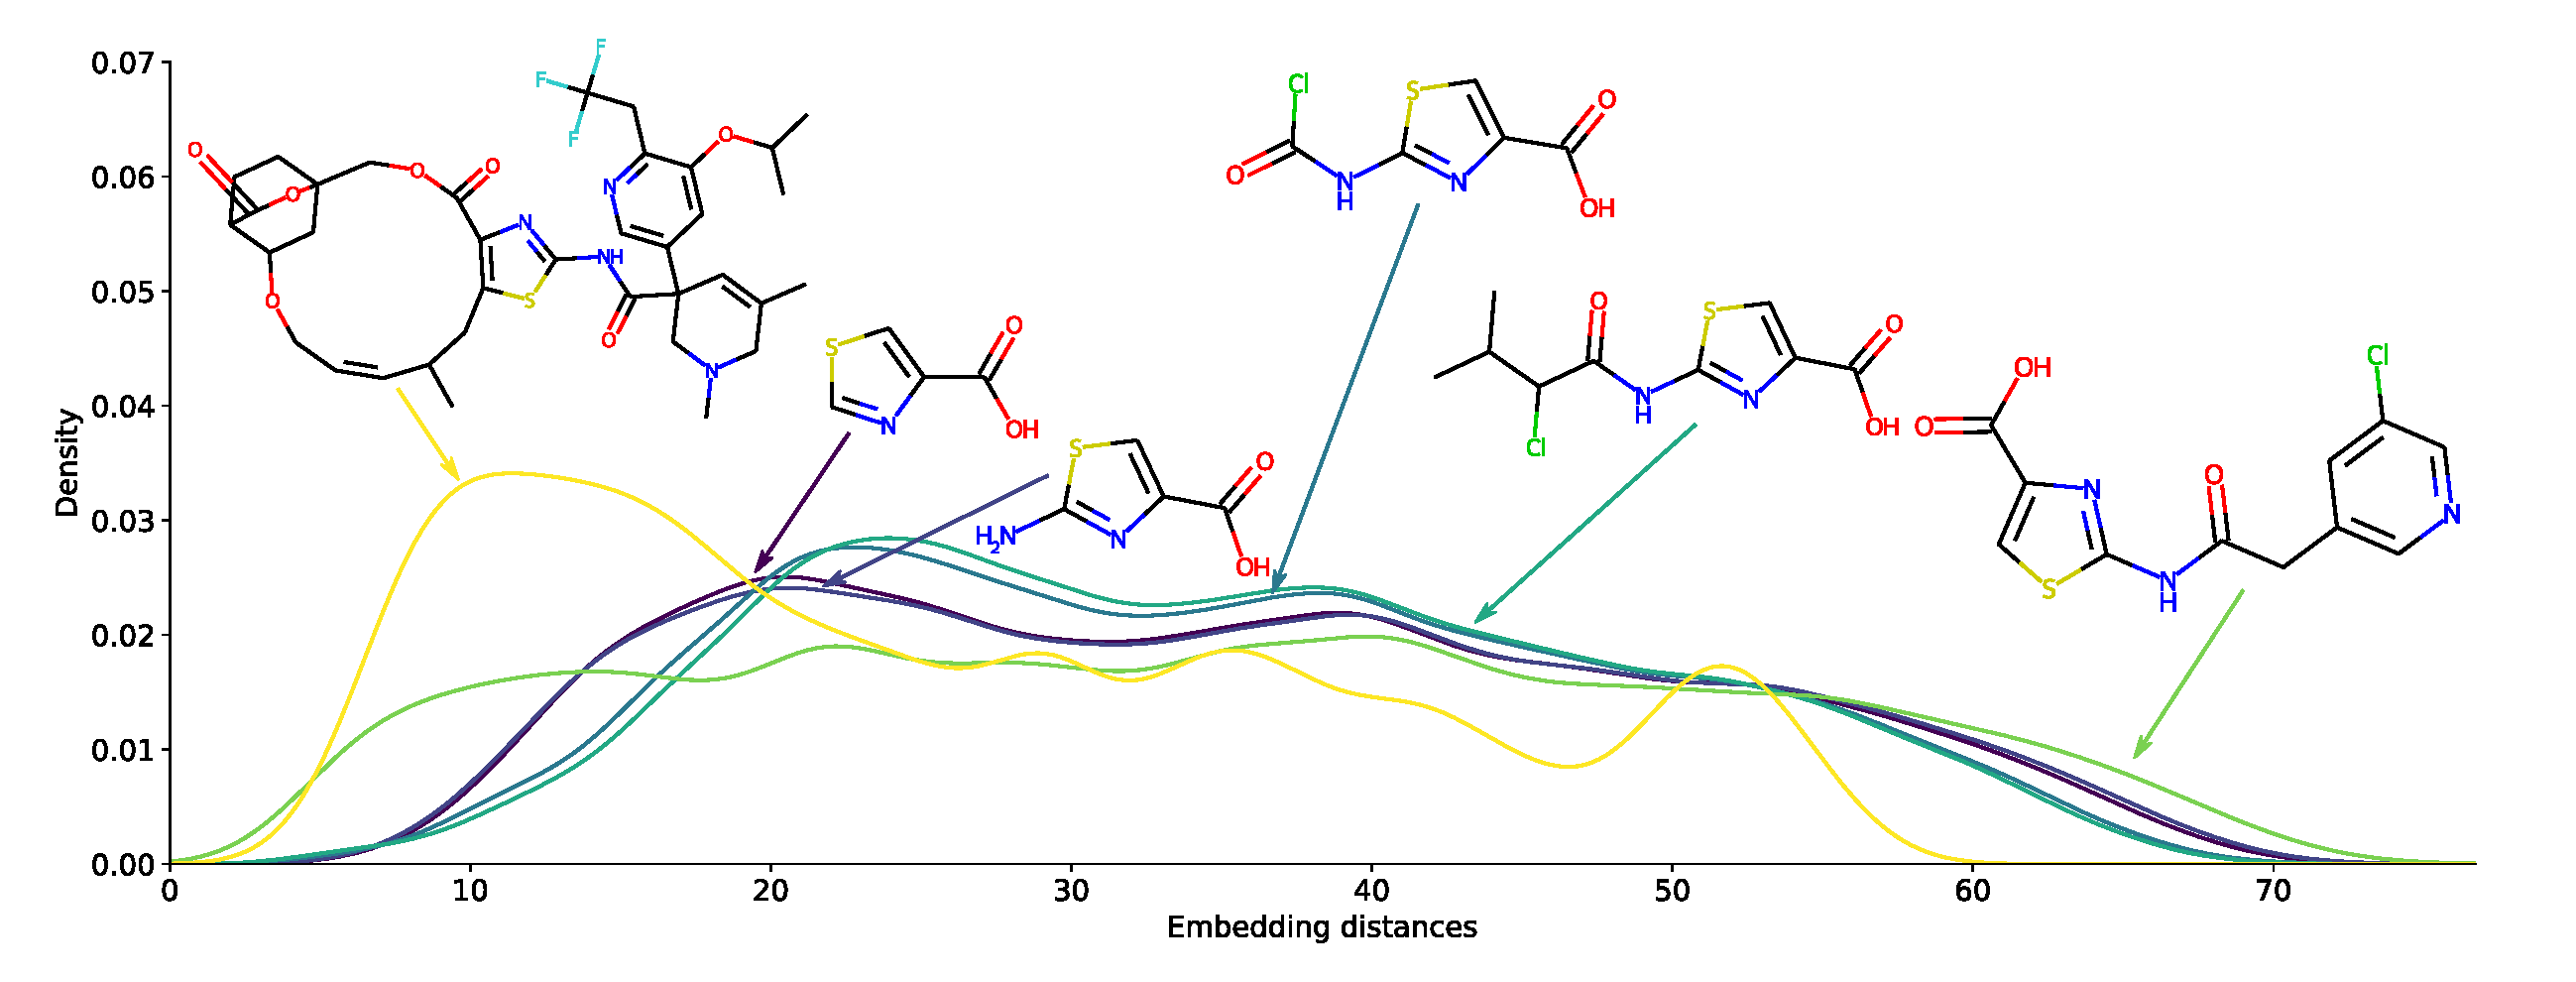
\includegraphics[width=\textwidth]{data/References_distributions.pdf}
\caption{Distribution of embedding distances of 5 references compounds to a diverse set of 120k compounds from the Zinc database.}
\label{fig:References_distributions}
\end{figure}


Another point where fingerprints fail to accurately describe molecular similarity is the case of molecules with repeated motifs. When using Tanimoto similarity of circular fingerprints in bit string form, the similarity tapers off quickly to a fixed non-zero value. The learned embedding is immune to this effect. Likewise, the insertion of moieties within a scaffold has an unduly small effect when it does not perturb the fragmentation of the structure by fingerprints, but is correctly shown to matter a lot by the embedding. In addition, it also retains the concepts of fragments, aromaticity, and some level of isosterism. Some examples illustrating these points are shown in Figure \ref{fig:Similarity_study_cases}.


\begin{figure}[hbtp]
\centering
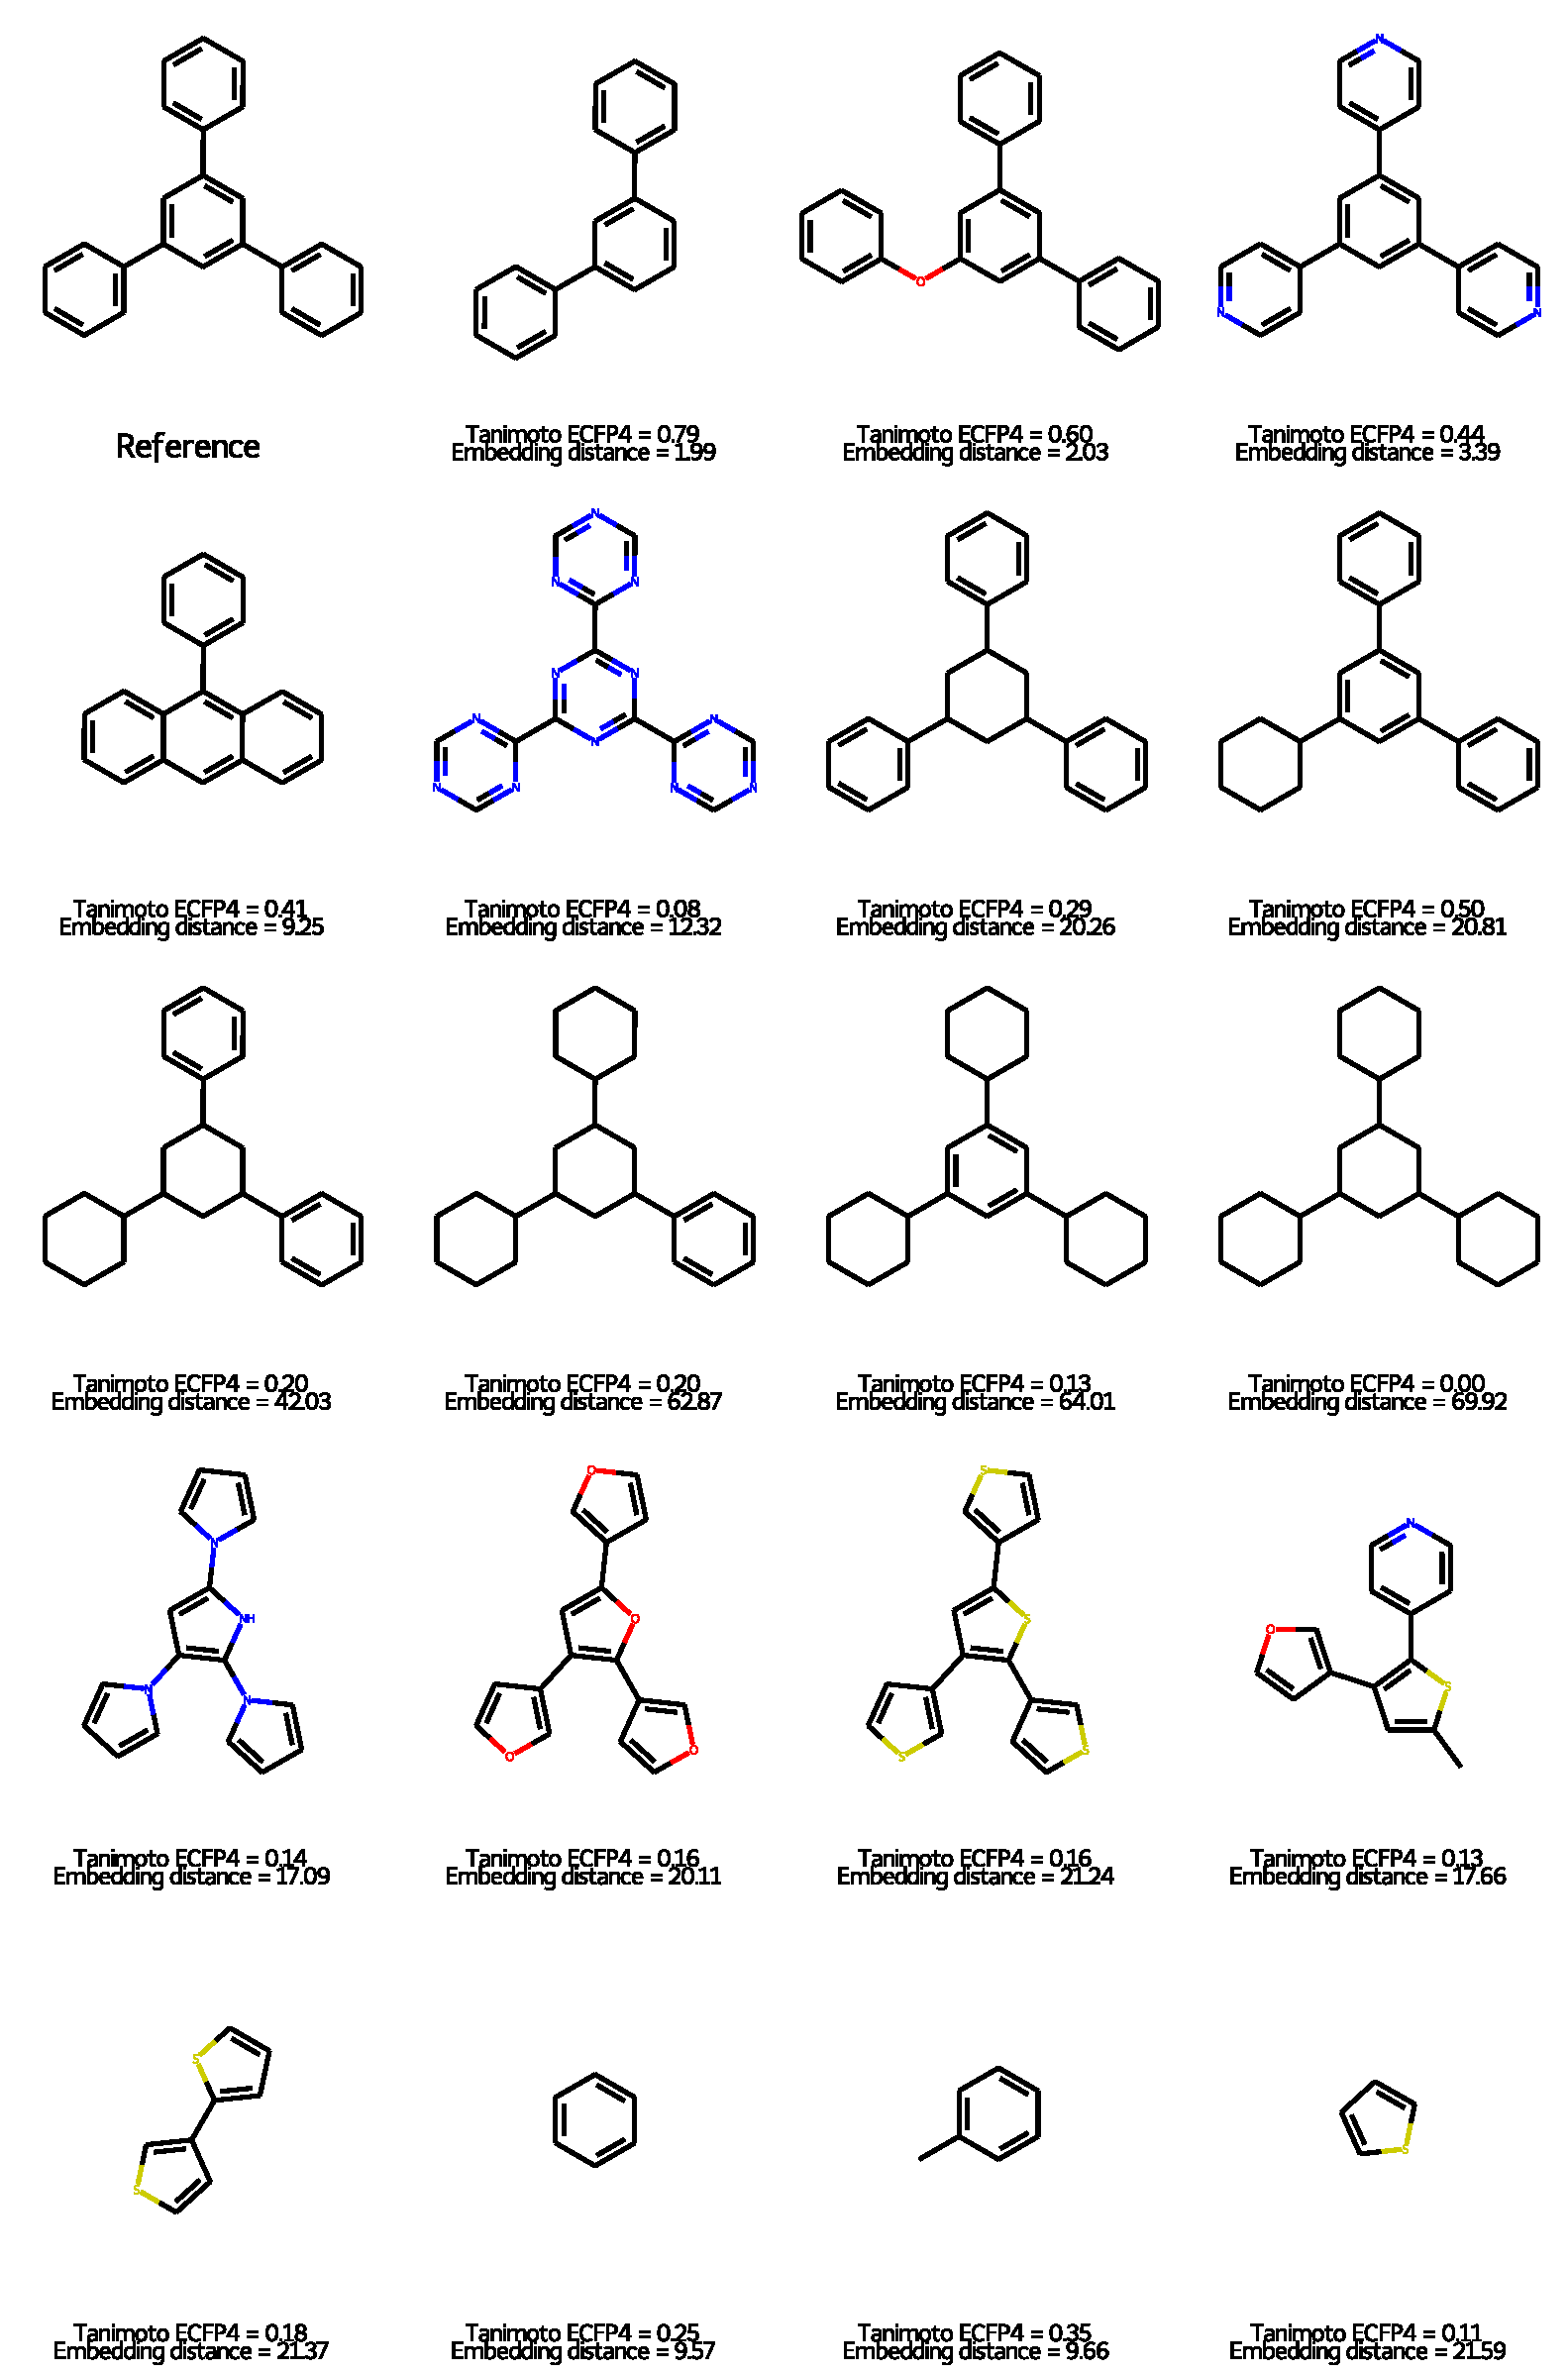
\includegraphics[height=\textheight]{data/Similarity_study_cases.pdf}
\caption{Selection of pairwise comparisons illustrating a diverse set of molecular similarities.}
\label{fig:Similarity_study_cases}
\end{figure}


\subsection{Additional properties}
As stipulated earlier, the distribution of similarities should be notably different between positive examples and negative examples: the first distribution should show a sharp peak around optimal similarity, and the second should display a long tail representing the many different sources of dissimilarity. After applying both the ECFP4 Tanimoto coefficient comparison and the learned MPNN embedding to unseen triplets of our generated dataset, we indeed see such a behaviour illustrated in \ref{fig:ECFP4_Embedding_triplets}.

\begin{figure}[hbtp]
\centering
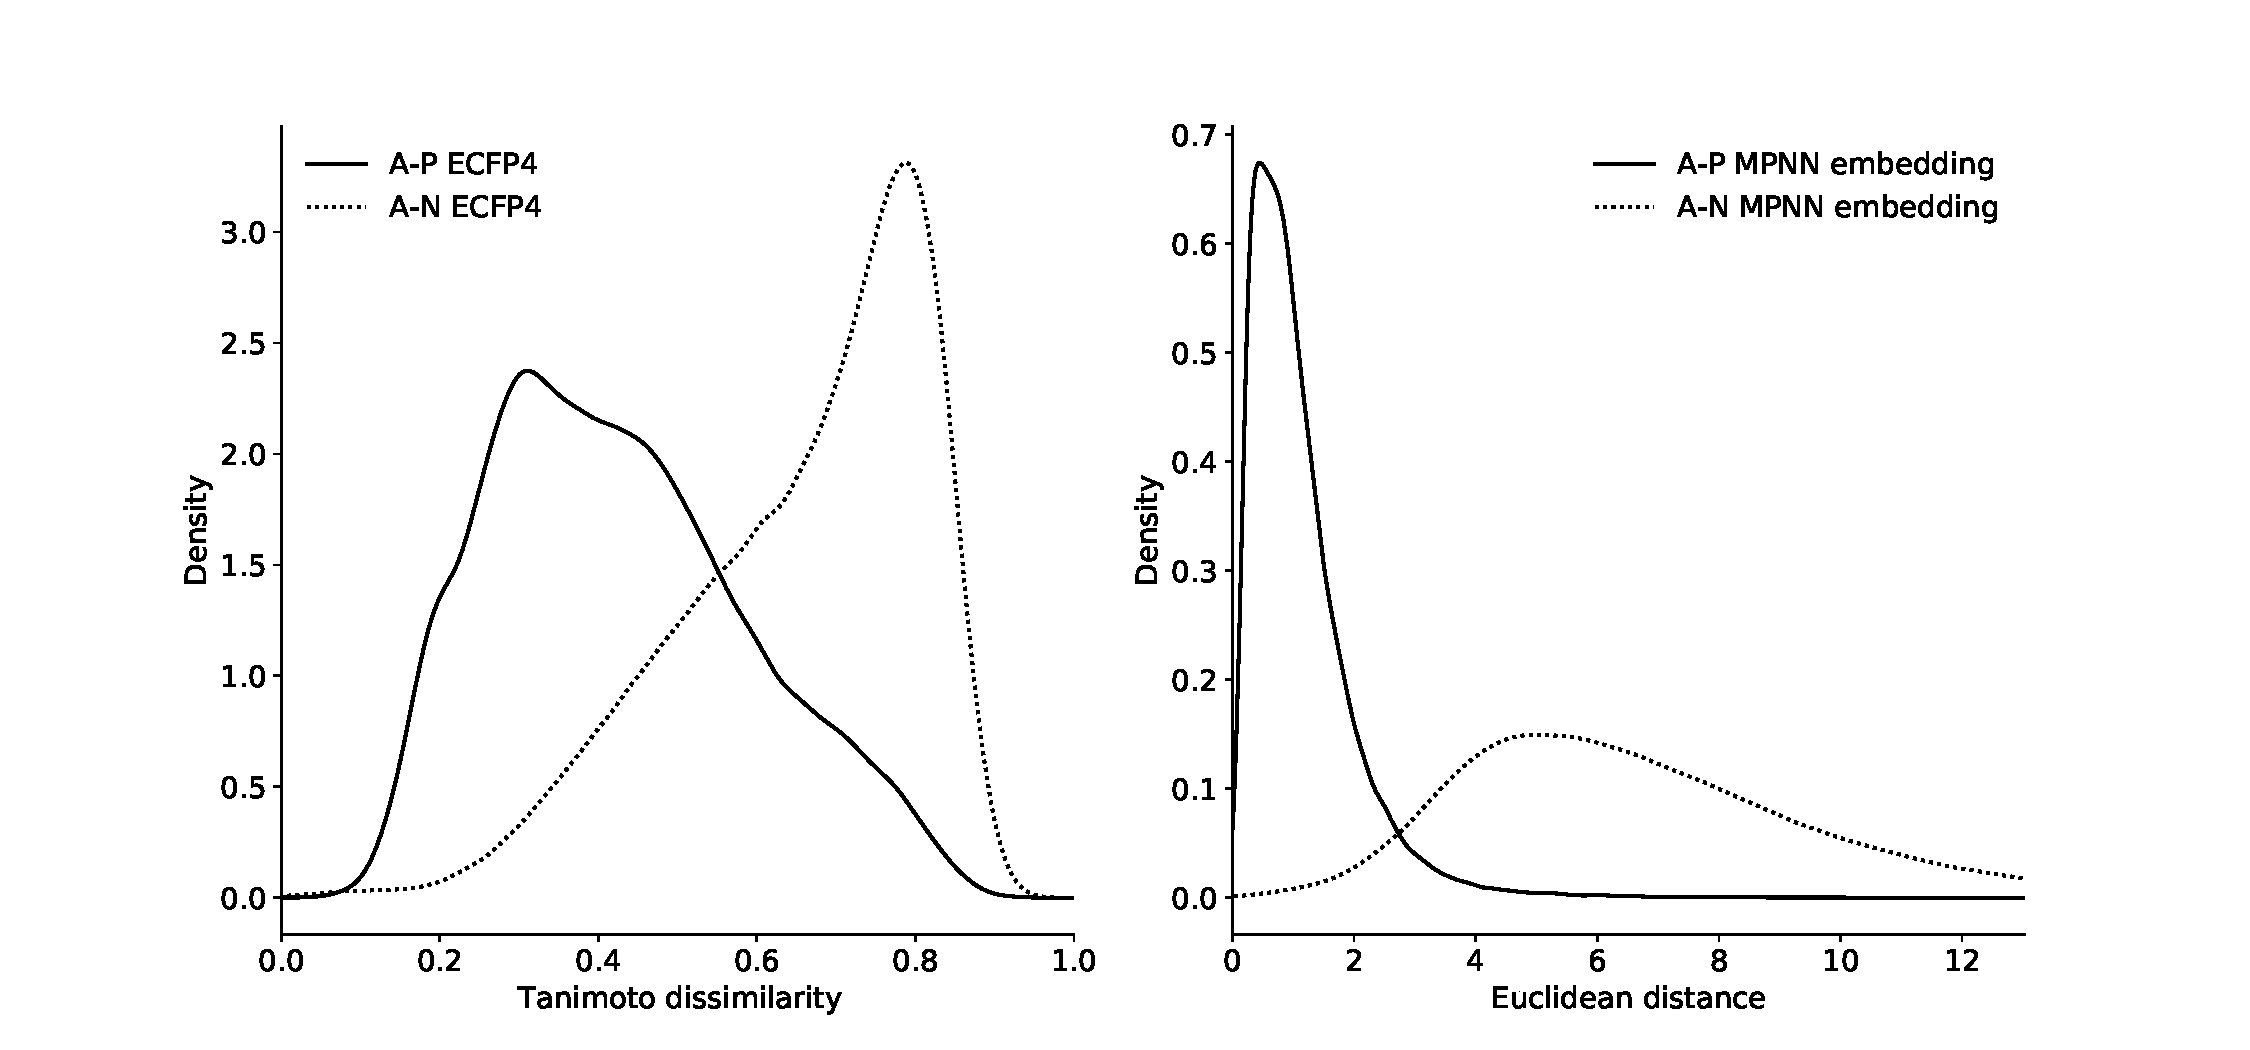
\includegraphics[width=\textwidth]{data/ECFP4_Embedding_triplets.pdf}\caption{Comparison of the similarity distributions on unseen triplets}
\label{fig:ECFP4_Embedding_triplets}
\end{figure}

Another critical desired property for a novel molecular distance measure is the ability to correctly compare partial and \emph{chemically invalid} molecular graphs and provide gradient information. This leads to the important fact that trained embeddings are essentially derivable reconstruction loss with a quadratic energy surface, with widespread potential applications. For example:
\begin{itemize}
\item Accelerated training of reconstruction based molecular generators such as variational auto-encoders.
\item Additional information in tasks such as missing edge and node prediction.
\item Chemical subspace constraints for conditional molecular generators
\end{itemize}
These tasks are deeply unsuitable to traditional fingerprints or property based similarity : for most of the training process, the molecular graphs on which computation happens are completely invalid, the chemical information on what is a molecule still being accrued. Yet a learned embedding, as is shown in Figure~\ref{fig:Ablations}, is very robust to node and edge deletion, demonstrating a quasi linear distance relationship with the number of deleted elements. This is an exciting property, and we look forward to seeing it explored further.

\begin{figure}[hbtp]
\centering
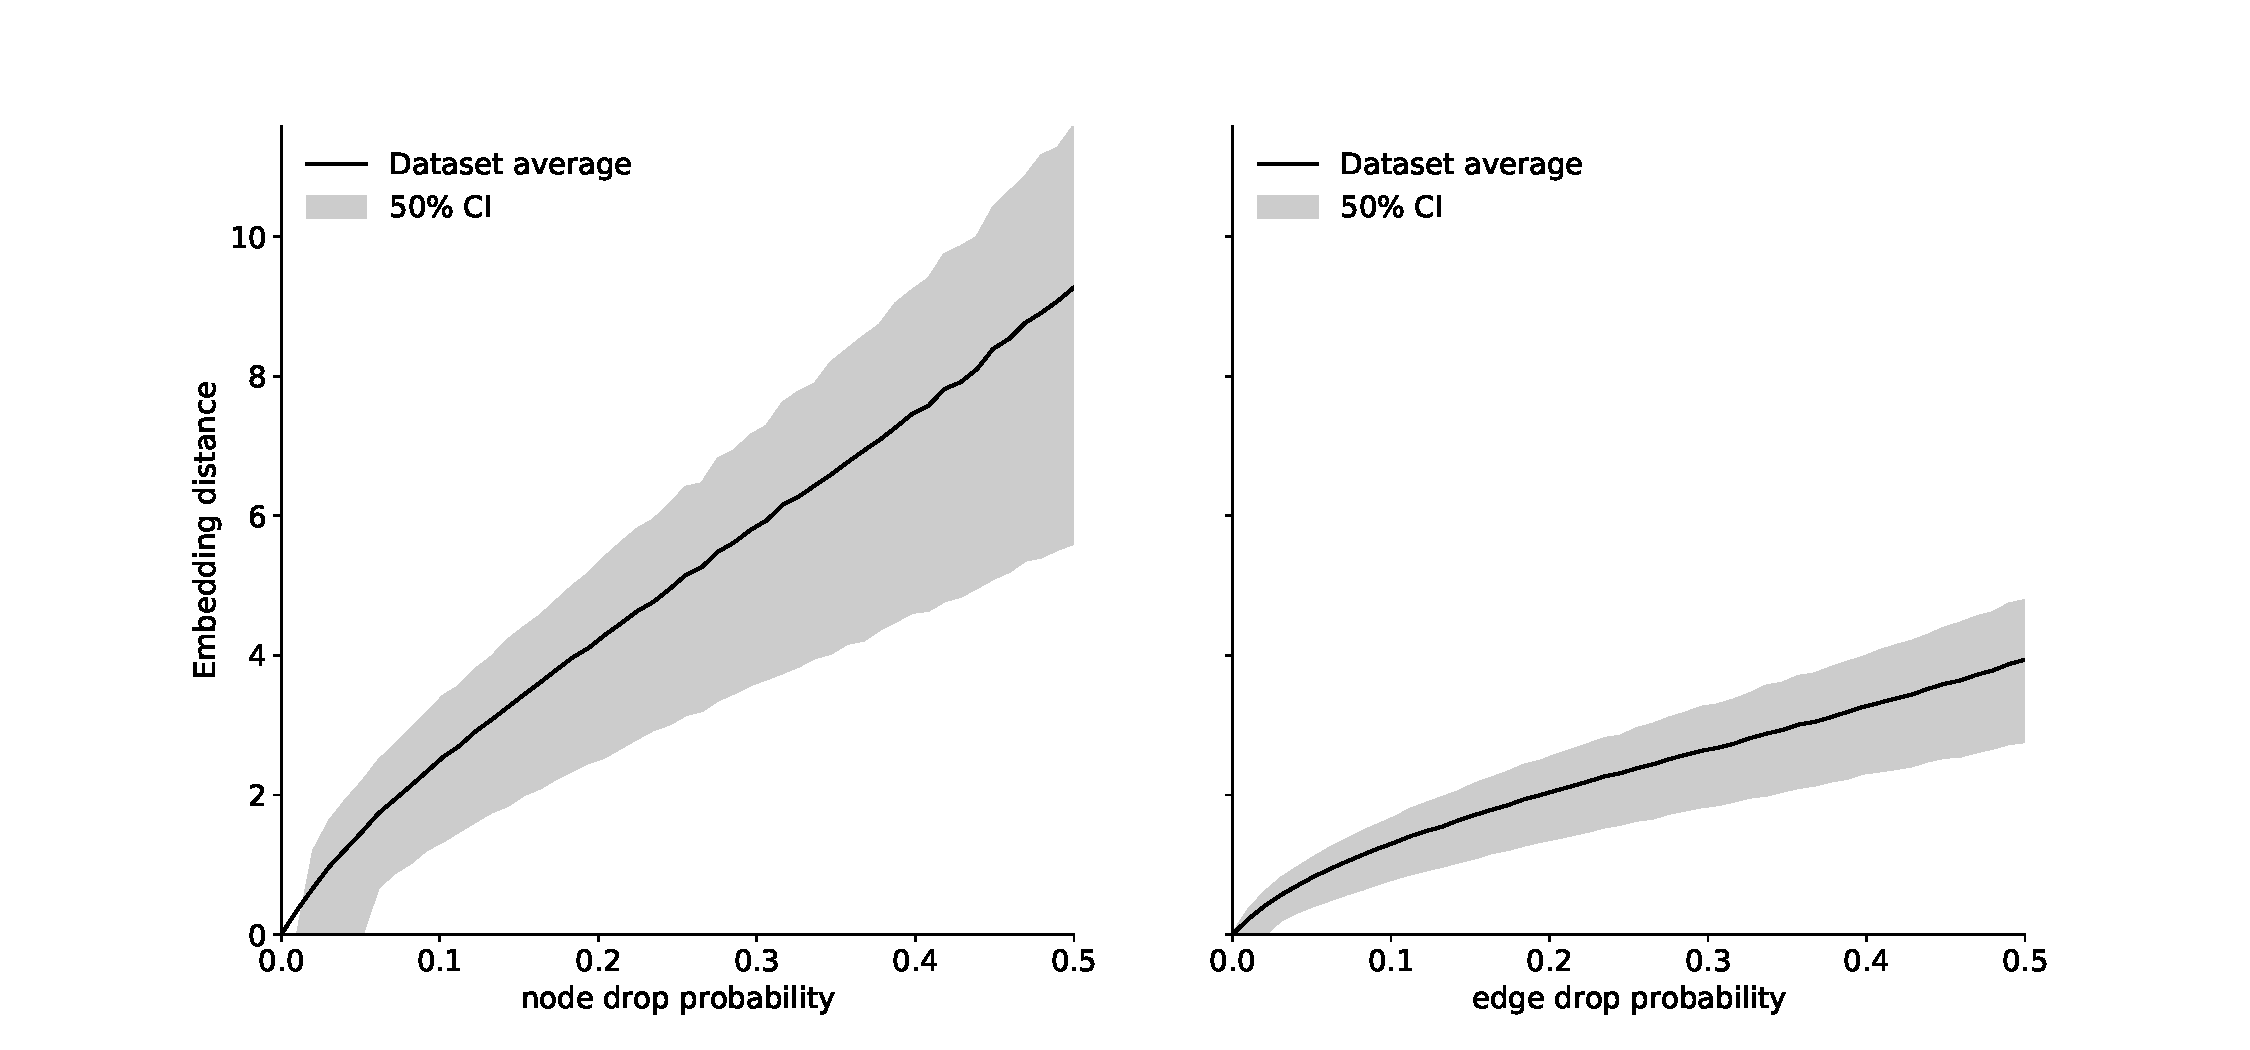
\includegraphics[width=\textwidth]{data/Ablations.pdf}
\caption{Effect of random element deletion on embedding distance. No comparison with ECFP4 could be obtained due to the overwhelming rate of invalidity of the resulting structures.}
\label{fig:Ablations}
\end{figure}

Finally, a critical property of the embedding is its ability to be used in conjunction with transfer learning\cite{tan2018survey, weiss2016survey}, and be retrained on particular subsets of the chemical space according to tailored similarities obtained from SAR, Molecular Matched Pairs\cite{griffen2011matched}, or a more complex multiple-parameters function. Such a retrained model would retain the general concepts of molecular graph similarity while quickly converging to a more appropriate representation of the problem at hand, thus sparing resources in training and data gathering.

\section{Conclusions}\label{conclusions}
We have shown that using the triplet margin loss jointly with molecular graph based deep neural networks trains latent representations that satisfy the many definitions of chemical similarity. A naive example of such an embedding was trained with no hyperparameters optimization on a dataset constructed from public molecules and some basic concepts of graph similarity. This naive example compares acceptably out of the box with the accepted standard of circular fingerprints Tanimoto scores, while possessing many additional properties such as being derivable or retrainable. We believe such properties may be of great use to train reconstruction based molecular generators. 

All code and data is available on github.com and is sufficient to reproduce our conclusions and graphs.

The authors were both employed by GlaxoSmithKline UK at the time of the present work.

\begin{acknowledgement}

The authors thanks Darren Green and Kim Branson for their preliminary review; as well as the entire Molecular Design team for their constructive feedback.

\end{acknowledgement}

\begin{suppinfo}

The following files are available free of charge.
\begin{itemize}
  \item lightning\_logs.zip: a compressed file containing the detailed training logs of the example model presented in this work. Visualize using the tensorboard utility, as described here: \href{https://pytorch-lightning.readthedocs.io/en/stable/starter/introduction_guide.html}{pytorch-lightning.readthedocs.io}
  \item model_trained.zip: the weights and hyperparameters checkpoint of the example model presented in this work. Should be used in conjunction with the code released on github.
\end{itemize}

\end{suppinfo}

%\bibliographystyle{abbrv}
\bibliography{chemdist}

\end{document}
This is never printed
